%%%%%%%%%%%%%%%%%%%%%%%%%%%%%%%%%%%%%%%%%%%%%%%%%%%%%%%%%%%%%%%%%%%%%%%%%%%%%%%%
%2345678901234567890123456789012345678901234567890123456789012345678901234567890
%        1         2         3         4         5         6         7         8

\documentclass[letterpaper, 10 pt, conference]{ieeeconf}  % Comment this line out
                                                          % if you need a4paper
%\documentclass[a4paper, 10pt, conference]{ieeeconf}      % Use this line for a4
                                                          % paper

\IEEEoverridecommandlockouts                              % This command is only
                                                          % needed if you want to
                                                          % use the \thanks command
\overrideIEEEmargins
% See the \addtolength command later in the file to balance the column lengths
% on the last page of the document



% The following packages can be found on http:\\www.ctan.org
\usepackage{graphics} % for pdf, bitmapped graphics files
\usepackage{epsfig} % for postscript graphics files
%\usepackage{mathptmx} % assumes new font selection scheme installed
%\usepackage{times} % assumes new font selection scheme installed
\usepackage{amsmath} % assumes amsmath package installed
\usepackage{amssymb}  % assumes amsmath package installed

\usepackage{url}
\usepackage[ruled, vlined, linesnumbered]{algorithm2e}
%\usepackage{algorithm}
\usepackage{verbatim} 
%\usepackage[noend]{algpseudocode}
\usepackage{soul, color}
\usepackage{lmodern}
\usepackage{fancyhdr}
\usepackage[utf8]{inputenc}
\usepackage{fourier} 
\usepackage{array}
\usepackage{makecell}

\SetNlSty{large}{}{:}

\renewcommand\theadalign{bc}
\renewcommand\theadfont{\bfseries}
\renewcommand\theadgape{\Gape[4pt]}
\renewcommand\cellgape{\Gape[4pt]}

\newcommand{\rework}[1]{\todo[color=yellow,inline]{#1}}

\makeatletter
\newcommand{\rom}[1]{\romannumeral #1}
\newcommand{\Rom}[1]{\expandafter\@slowromancap\romannumeral #1@}
\makeatother

\pagestyle{plain} 

\title{\LARGE \bf
Intrusion Detection Framework for Home Automation using Computer Vision and Honeypot 
}

%\author{ \parbox{3 in}{\centering Huibert Kwakernaak*
%         \thanks{*Use the $\backslash$thanks command to put information here}\\
%         Faculty of Electrical Engineering, Mathematics and Computer Science\\
%         University of Twente\\
%         7500 AE Enschede, The Netherlands\\
%         {\tt\small h.kwakernaak@autsubmit.com}}
%         \hspace*{ 0.5 in}
%         \parbox{3 in}{ \centering Pradeep Misra**
%         \thanks{**The footnote marks may be inserted manually}\\
%        Department of Electrical Engineering \\
%         Wright State University\\
%         Dayton, OH 45435, USA\\
%         {\tt\small pmisra@cs.wright.edu}}
%}

\author{Aadhaar Koul , Arjun Charak , Baseer Fatima , Navneet Kour% <-this % stops a space 
\\ Department of Computer Science and Engineering \\
Model Institute of Engineering and Technology \\
Kot Bhalwal , Bantalab , Jammu and Kashmir , India \\
{\tt\small\{2020a1r040, 2020a1r058, 2020a1r048, 2020a1r045\}@gmail.com} \\ \\
% Dr. Geetha V%
% \\ Department of Information Technology \\
% National Institute of Technology Karnataka \\
% Surathkal, Mangaluru 575025, Karnataka, India \\
% {\tt\small geethav@nitk.edu.in}
}


\begin{document}



\maketitle
\thispagestyle{plain}
\pagestyle{plain}



%%%%%%%%%%%%%%%%%%%%%%%%%%%%%%%%%%%%%%%%%%%%%%%%%%%%%%%%%%%%%%%%%%%%%%%%%%%%%%%%
\begin{abstract}
Internet of Things (IoT) represent a network of resource-constrained sensor devices connected through the open Internet, susceptible to misuse by intruders. Traditional standalone intrusion detection systems (IDS) are tasked with monitoring device behaviours to identify malicious activities. These systems not only require extensive network and system resources but also cause delays in detecting a malicious actor due to unavailability of a comprehensive view of the intruder's activities.Collaboration among IoT devices enables considering knowledge from a collection of host and network devices to achieve improved detection accuracy in a timely manner. However the collaboration among the IOT devices may create a bundle of alert messages at the time of intrusion. In this paper we present a new approach to intrusion detection system through a collaborative framework that leverages the security oriented techlonogies such as honeypot systems and Artificial intelligence to generate less network traffic and optimized alerts. The paper presents a detailed formal description of the proposed framework along with analysis to assess its effectiveness for a typical Home Automation system. We implemented the CHAKRAVYUH framework with Raspbian OS and conducted thorough experimentation to evaluate its performance. The evaluation demonstrates efficiency of CHAKRAVYUH framework with respect to energy and processing overheads achieving effectiveness within an IoT system.

\end{abstract}

\begin{keywords}


\end{keywords}

%%%%%%%%%%%%%%%%%%%%%%%%%%%%%%%%%%%%%%%%%%%%%%%%%%%%%%%%%%%%%%%%%%%%%%%%%%%%%%%%
\section{INTRODUCTION}
Over the past decades, Internet and computer systems have raised numerous security issues due to the explosive use of networks. CERT statistics (CERT) reports that the amount of intrusions has excessively increased year by year. Any malicious intrusion or attack on the network vulnerabilities, computers or information systems may give rise to serious disasters, and violate the computer security policies, i.e., Confidentiality, Integrity and Availability (CIA). Up to now, the threats on network and information security are still significant research issues. Though there is a number of existing literatures to survey IDS and its taxonomy (Denning, 1987, Lunt, 1993, Mukherjee et al., 1994, Debar et al., 1999, Axelsson, 2000, Mishra et al., 2004, Krugel and Toth, 2000, Jones and Sielken, 2000, Debar et al., 2000, Mukkamala and Sung, 2003, Estevez-Tapiador et al., 2004, Delgado et al., 2004, Kabiri and Ghorbani, 2005, Anantvalee and Wu, 2007, Patcha and Park, 2007, Tucker et al., 2007, Mandala et al., 2008, Garcia-Teodoro et al., 2009, Amer and Hamilton, 2010, Xie et al., 2011), we try to give a more systematic, architectural and contemporary image for a comprehensive review. \\

At first we take a look at the already existing work that been done over the years on the topic of intrusion Detection Framework. F. Cuppens; A. Miege 's research work done on the intrusion detection framework proposes the idea of a collaborative framework that leverages the power of the collaborative modules in the IOT that share data to each other and deliver the alerting messages in the form of bundles that are then formulated and parsed in order to serve the relevant data to the admin. Every alert is modeled using the IDMEF format. A Document Type Definition (DTD) has been proposed to describe IDMEF data format through XML documents. This is the representation we shall
consider in the remainder of this paper. However, the correlation function does not directly deal with this XML representation of alerts. It is actually
automatically converted into a set of logical facts. This set
of facts is then stored in a database. \cite{c7}\\

Another methodology proposed by (Reda M. Elbasiony, Elsayed A. Sallam 1, Tarek E. Eltobely 2, Mahmoud M. Fahmy ) proposes a different approach stating to implement an Intrusion Detection Framework based on random forests and weighted k-means which works on the principle of data mining classification and clustering techniques. This technique uses the random forests classification algorithm is used to build intrusion patterns automatically from a training dataset, and then matches network connections to these intrusion patterns to detect network intrusions. 

\begin{equation}
W(S,C) = \sum_{k=1}^{K}  \sum_{i \in I}  \sum_{v=1}^{M} [S_{ik}(y_{iv} - c_{kv})(y_{iv} - c_{kv})]
\end{equation}

where sik = 1 if i ∈ sk, and sik = 0, otherwise \\

Lastly we took a look at the methodology proposed by (Junaid Arshad, Muhammad Ajmal Azad, Mohammad Mahmoud Abdellatif, Muhammad Habib Ur Rehman, Khaled Salah
) that proposes a collaborative intrusion detection framework (COLIDE) for IoT leveraging collaboration among resource-constrained sensor and border nodes for effective and timely detection of intruders. The paper presents a detailed formal description of the proposed framework along with analysis to assess its effectiveness for a typical IoT system. They have  implemented the COLIDE framework with Contiki OS and conducted thorough experimentation to evaluate its performance. The evaluation demonstrates efficiency of COLIDE framework with respect to energy and processing overheads achieving effectiveness within an IoT system. \\

In this paper we have formulated a detailed description on the proposed framework that covers the methodology , concepts , framework , workflow , workdone . Based on which the estimation and results have been formulated. Many current IDSs are rule-based systems that depend on a set of rules representing attacks or normal network characteristics, which are collected and identified by security experts.This paper proposes a hybrid IDS based on two famous algorithms called YOLO V7, and Deep KNN. We  propose a near-end strategy optimization method for Industrial IoT intrusion detection system using computer vision and honeypot technology. The system integrates network gateway, Blynk cloud, and Android application to present
relevant information. Deep KNN, feature selection based on Light GBM and ReLU activation function are used to construct the intrusion detection model. The proposed system achieves a high detection rate of 97 percent for various parameter assaults and out performs existing intrusion detection systems based on deep learning models. The proposed 
system provides a robust and efficient solution for detecting network assaults in real time. In the Honeypot part of our framework, Canary Tokens are used to classify network connections into intrusion and normal data based on labeled  classification patterns , but here we have impleentes the canary tokens solely for the pourpose of an intrusion in the IOT module specifically the honeypot module which will then be integrated into the user end mobile device. \\

The reminder of this paper is organized as follows. We describe IDS methodologies in Section 2, and the classification of IDS approaches in Section 3. Section 4 introduces four classes of IDS technologies. We study IDS issues on VMs in Section 5. Subsequently, two software-oriented solutions, Snort and ClamAV, are studied in Section 6, as they are most widely used open-source tools. Section 7 draws our conclusion, and gives future challenges.



\section{LITERATURE SURVEY}
In this section, we present the basic concepts used throughout the rest of this paper which are important to understand the proposed system. Furthermore, we include an attack model identifying the threats addressed by the CHAKRAVYUH framework.

\subsection{Background and Threat Model}
\subsubsection{IPv6 over Low-Power Wireless Personal Area Networks (6LoWPAN)}
IPv6 over Low-Power Wireless Personal Area Networks (6LoWPAN) is a networking protocol designed to address the unique challenges of integrating Internet Protocol version 6 (IPv6) communication within low-power, resource-constrained wireless networks. These networks are frequently utilized in various Internet of Things (IoT) applications, where devices need to communicate over short distances while conserving energy. Despite its advantages, 6LoWPAN faces several challenges. Ensuring data security and privacy in resource-constrained environments is a concern due to limitations on implementing robust encryption and authentication mechanisms. Interoperability can be complex due to the diversity of devices and protocols used in IoT networks. As the number of connected devices grows, scalability becomes an issue for routing and addressing mechanisms within 6LoWPAN-enabled networks.\cite{c8}\\

\subsubsection{Threat model for the IoT}
Although the IoT is an emerging paradigm, a significant part of the software stack used by the IoT applications is adopted from the existing computing paradigms. This is also evident from the integration of IoT specific stack (such as specific to 6LoWPAN and RPL) [15] with the existing Internet infrastructure such as IPv4 and IPv6. Consequently, an attack model for IoT infrastructures is not restricted to the threats specific to the new routing protocols such as 6LoWPAN and RPL but also includes threats to existing infrastructure such as IPv6, application specific attacks, and attacks specific to the physical media such as the radio spectrum.
\begin{figure}[thpb]
      \centering
      {\parbox{2.8in}{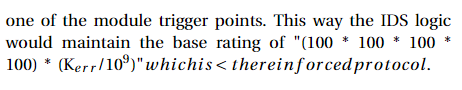
\includegraphics[height=1.5in, width=2.8in]{Images/2.png}}}
      \caption{Attack Model for IoT Network}
      \label{fig:2}
\end{figure}

Our research is aimed at developing a collaborative intrusion detection system for IoT infrastructures using AI and honeypots. Therefore, we focus on three  types of threats for this paper, i.e. physical , routing-specificand software specific threats. As The proposed system is a software entity, we render the threats at the physical layer out of the scope of this research. \\

\subsubsection{Physical Aspect}
Routing attacks directly impact the low-power devices and their routing tables. This can be achieved by making the flooding or denial of service (DoS) attacks with respect to routing tables. Potential routing attacks for an IoT system are presented below.\\

Rank attack: 6LoWPAN networks use ranking to establish an optimal routing path. Within this context, Node Rank indicates the quality of the path from a node to the sink node. Every time a node updates its rank or preferred parent, it needs to inform other nodes by sending the updated information in the next cycle. RPL uses the rank rule such that a node in the parent should always have a lower rank than its children to prevent the loop creation. This enables creating an optimal topology, preventing loop creation and managing control overhead [16]. As identified by [16-18], the rank information can be maliciously tampered with by an attacker so that it chooses the node with worst rank to be its parent. This will result in disrupting the topology of the network causing delays in normal transmission.\cite{c8}
Wormhole attack: A wormhole can be considered as a tunnel between two nodes using wired or wireless links and can be used to achieve faster transmission rates or dedicated connection between such nodes. As such, a wormhole has legitimate applications such as the connection between the local and global IDS modules within our architecture. However, a wormhole as identified by [19] can be used by an attacker to create a dedicated tunnel with a node on the Internet. Wormhole attack is not novel to the IoT networks and has been historically identified as a potential threat for wireless sensor networks (WSN) [20-22].
Sinkhole attack: The objective of a sinkhole attack is to attract traffic through a designated node using illegitimate information making the node a lucrative routing sink (base station within wireless network terminology). As with wormhole attack, literature around sinkhole attack is well established with [23] being an initial effort to identify and mitigate against such attack. Creating a sinkhole does not necessarily disrupt legitimate transmission within a 6LoWPAN. However, diverting the traffic through a specific route creates opportunities to launch other attacks such as wormhole and selective-forwarding attack described below.
Selective-forwarding attack: With selective-forwarding attack, a malicious node attempts to disrupt legitimate transmission and routing path. The malicious node, in this case, attempts to block certain packets and forward selected packets thereby affecting the routing. For instance, an attacker can forward all RPL control messages but block the rest [19]. This attack can cause more damage when used in conjunction with a sinkhole attack. Such dependencies among different attack types have motivated us to explore the impact of multi-stage attacks within IoT infrastructures. To the best of our knowledge, the intrusion detection system presented in this paper is a pioneering effort to identify this issue and explore a solution to mitigate against it especially for IoT systems.
Fragment duplication attack: The fragment duplication attack leverages a weakness within the 6LoWPAN layer with respect to how fragmented packets are received and assembled by an IoT node. A consequence of the integration of 6LoWPAN with IPv6 networks is that bigger packets supported by IPv6 have to be fragmented into smaller packets so as to be effectively processed by the resource-constrained nodes within an IoT system. However, as identified by [24], a recipient node cannot verify if two fragments of a packet were sent from the same source. Therefore, the recipient node is unable to distinguish between legitimate and spoofed fragments. A malicious node can exploit this vulnerability to block reassembly of targeted packets such as connection establishment packets. This may result in disrupting legitimate traffic as well as depleting resources available to the victim node.
Buffer reservation attack: The buffer reservation attack is closely linked to the fragment duplication attack and may be caused as a consequence of a successful fragment duplication attack. The buffer reservation attack also targets the vulnerability in the fragmentation mechanism employed by 6LoWPAN networks. As identified by [24], it leverages the fact that the recipient of a fragmented packet is unable to determine if all fragments will be received correctly. Therefore, a recipient node reserves a buffer space based on the information provided in the 6LoWPAN header with any additional fragments discarded. Taking advantage of this setting, a malicious node can send its victim single F RAG1 to reserve arbitrary buffer space thereby consuming scarce memory of the resource-constrained node.
Sybil and clone ID attack: Sybil and clone ID attacks are similar in that the objective of the attacker is to use spoofed logical identities within a network without deploying physical devices. In particular, for clone ID attack, an attacker is aiming to use a victim's logical identity within the network. Whereas, in Sybil attack, the attacker aims to assume multiple logical identities within a network without deploying physical nodes. These logical identities may not be currently present in the network. A number of existing efforts such as [19, 23] have identified these attacks for IoT and historically for WSNs. \cite{c8}\\

\subsubsection{Application of specific threats}
In addition to routing-specific threats mentioned above, IoT infrastructures are susceptible to other types of threats such as application specific threats. Although routing forms an essential component of the IoT system, the IoT devices are expected to run application software required by the function envisaged to be performed. We categorise these threats as application specific and present them below. \\

DoS attack: Historically, DoS attacks are used to make the victim unavailable for legitimate service. This can be achieved via flooding the victim with the extraordinarily large volume of requests or by exhausting the resources such as memory and computational power available to the victim. Within IoT, the threat of DoS attack is two-fold: the victim can be part of the network under threat that an attacker wishes to make unavailable or the victim can be used as a zombie (stepping stone) to launch a Distributed DoS (DDoS) on a target IoT network. The significance of these threats within IoT systems has been identified by [25-27]
Malicious code injection: As identified by [26, 28], malicious code injection is another application specific threat to IoT systems. The attacker, in this case, attempts to inject malicious code to get privileged access to the victim. Consequently, the attacker can damage the normal operation by causing a threat to the data or to the network using one of the routing-specific attacks described in the previous section.
Traditional subversion attacks: In addition to the above-mentioned attacks, IoT systems are vulnerable to the existing attacks targeted at computer systems such as message interception, fabrication, modification, subversion, phishing, etc. As with the routing-specific attacks, these attacks can also form a part of a more complicated and sophisticated attack. \\

\subsubsection{Intrusion detection within IoT systems}
Intrusion detection is a vital aspect of securing Internet of Things (IoT) systems, which bring convenience and efficiency through interconnected devices. Intrusion detection involves monitoring and analyzing network activities to identify unauthorized or abnormal behavior, ensuring data integrity and availability. However, IoT systems pose unique challenges, including resource constraints in devices, network heterogeneity, scalability, and diverse data volumes. Two main detection approaches exist: signature-based detection using predefined attack patterns, and anomaly-based detection relying on deviations from normal behavior. The future of IoT intrusion detection lies in incorporating machine learning and artificial intelligence for adaptive defense, improving behavioral analysis, and fostering collaborative defense mechanisms to counter emerging threats. This evolving field is critical for maintaining the security and privacy of interconnected IoT environments. \\

\subsection{CHAKRAVYUH Framework}
A Framework in which the modules computer vision , surveillance , Blynk cloud, IOT , network gateway , Honeypot , android application work in a coordinatedmanner . the framework would comprises of a Network and home automation control
panel that is receiving real-time responses from different components like wifi , detection sensors , arduino , home gateway , media server . The wifi render theinformation from a centralized home security system that comprises of a VPN, Network Sniffer , IP surveillance and a honeypot system. The detection sensors
receive information from the ultrasonic sensors , laser sensors , motion sensors , PIRsensors in real-time. The arduino renders the real-time information from electricity appliances. the home gateway renders the information from the home gateway dashboard and a media server the is connected to the network storage. ..... whenever at
any instant a sensor or an activity happens on any of the modules of the frameworkaSmart notification system triggers a push notification in the admin control applicationtelling them that there has been an intrusion on a particular sensor. 

\begin{figure}[thpb]
      \centering
      {\parbox{2.8in}{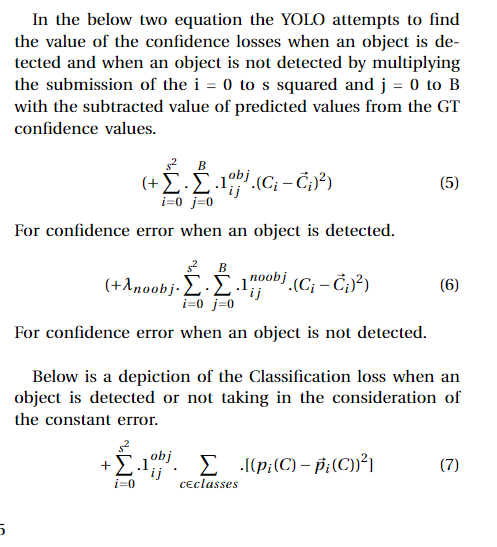
\includegraphics[height=1.5in, width=2.8in]{Images/3.png}}}
      \caption{CHAKRAVYUH Framework}
      \label{fig:2}
\end{figure}

The framework proposed here uses a collaborative module Threat level based algorithm that assigns a base level rating to all the trigger points , combines them and classifies the threat level into three level of intrusion. \\
The way this works is that the algorithm quantifies the threat level ratings from the trigger points such as the network gateway , IOT modules , survelliance modules , AI detection module or the honeypot system and binds them into an equation that when divided by a constant scaled down number makes it much more calculatable (Lower scale number). This allows us to segergrate the threat level into three of the threat levels such as : \\ \\
Level 1 : Standard Protocols : value = 1500 \\
Level 2 : Reinforced Protocols : value = 2100 \\
Level 3 : Strict Protocols : value = 6250 \\

The Above levels describe the level of intrusion between their respected ranges that limits under an overall rating of 10000. \\

\begin{equation}
TL = [{(\sum_{Tp_1=0}^{Tp_1=1K} . \sum_{Tp_2=0}^{Tp_2=1K} . \sum_{Tp_3=0}^{Tp_3=1K} . \sum_{Tp_4=0}^{Tp_4=1K}) (K_e_r_r / 10^9)}]
\end{equation}

In the aboe equation we are calculating the value of the threat level by combining all the realtime trigger point values withe constant error rate of K and scaling it down by a larger factor.\\ \\
For the equation to work we had to assign the base threshold value of the threat level to each and every one of the module trigger points. This way the IDS logic would maintain the base rating of "{(100 * 100 * 100 * 100) * (K_e_r_r / 10^9)}"
which is < the reinforced protocol.




\subsection{Computer Vision Module}
\subsubsection{Image Segmentation Performed by YOLO V.8}
Image segmentation is the task of partitioning an image into multiple regions or
segments, where each segment corresponds to a specific object or region of interest. YOLOv8 is a popular object detection algorithm that can be adapted for imagesegmentation. In the context of YOLOv8, the network is initially trained to performobject detection. It learns to predict the location and class of objects in an image by dividing the imageinto a grid and assigning bounding boxes to objects present in each grid cell. This
training process involves optimizing the network's parameters to minimize thedifference between predicted bounding boxes and the ground truth bounding boxes.To generate a segmentation mask, the predictions made by YOLOv8 are used. Eachbounding box prediction consists of the coordinates of the bounding box andthepredicted class of the object within it. These predictions are then utilized to determinethe pixel-level boundaries of each object. One common approach is to associate each pixel within a bounding box withthecorresponding object class. This can be achieved by assigning a specific value or label
to all pixels within the bounding box region. For example, if the object withinabounding box is a car, all pixels within that box are labelled as "car" inthesegmentation mask. However, a single bounding box may not cover the entire extent of an object, especially if the object is large or irregularly shaped. To handle this, additional
techniques can be applied to refine the segmentation mask. For instance, post- processing methods such as contour detection or region growing algorithms canbeutilized to expand the segmented regions based on the boundaries defined bythebounding boxes. \\ \\
Significant enhancements have been introduced to improve object detection performance. One major improvement is the addition of Batch Normalization on all convolutional layers, which aids convergence and reduces overfitting. The architecture consists of 24 convolutional layers, a combination of 3x3 and 1x1 convolutions, generating a 7x7 grid with 30 values per grid cell for bounding box and category predictions. High-resolution classification, achieved by fine-tuning with 448x448 ImageNet data, further refines YOLO v8's capabilities. The architecture is fully convolutional, utilizing anchor boxes for precise bounding box prediction. Dimension clustering and direct location prediction enhance accuracy, while finer-grained features and multi-scale training make it adaptable to different input sizes. \\ YOLO v8 brings about substantial improvements in object detection. It incorporates Batch Normalization, high-resolution classification, anchor boxes, dimension clustering, and direct location prediction. Additionally, it employs finer-grained features and multi-scale training for enhanced flexibility across various input sizes, making it a robust choice for object detection tasks.\cite{c1}\\

The functioning of the YOLO model depends upon the current state of a frame at a given instant of time which is dervied by subtracting the predicted value from the current value. The depiction of the above statement can be represented as follows. \cite{c2}\\
\begin{equation}
(\lambda_c_o_o_r_d . \sum_{i=0}^{s^2} . \sum_{j=0}^{B} . 1_{ij}^{obj})((x_i-\vec{x}
)^2 + (y_i - \vec{y})^2)
\end{equation}
The Lambda Coord here is set to 5 to increase the loss of bounding box predictions , the submission of 0 minus S squared is the sum value of each of the grid cell , The submission of 0 - B is  the value for each grid box further more YOLO is squaring the value gained by subtracting the Predictied bbox X-coordinate in the cell from the GT box x-coordinate in the cell added to the y coordinates of the same.

\begin{equation}
(+\lambda_c_o_o_r_d . \sum_{i=0}^{s^2} . \sum_{j=0}^{B} . 1_{ij}^{obj})((\sqrt{\omega}_i} - \sqrt{\vec\omega})^2 + ((\sqrt{h}_i} - \sqrt{\vec h_i})^2)
\end{equation}
In the above equation YOLO folows the same procedure but takes in consideration the height h in order to calculate the localization loss. \\ \\
NOTE : Eq 3 and 4 are both being used to find out the Localization loss in the YOLO. \\ \\

In the below two equation the YOLO attempts to find the value of the confidence losses when an object is detected and when an object is not detected by multiplying the submission of the i = 0 to s squared and j = 0 to B with the subtracted value of predicted values from the GT confidence values.

\begin{equation}
(+ \sum_{i=0}^{s^2} . \sum_{j=0}^{B} .  1_{ij}^{obj} . (C_i - \vec{C_i})^2 )
\end{equation}
For confidence error when an object is detected.\\
\begin{equation}
(+\lambda_n_o_o_b_j .  \sum_{i=0}^{s^2} . \sum_{j=0}^{B} .  1_{ij}^{noobj} . (C_i - \vec{C_i})^2 )
\end{equation}
For confidence error when an object is not detected.\\

Below is a depiction of the Classification loss when an object is detected or not taking in the consideration of the constant error.
\begin{equation}
+ \sum_{i=0}^{s^2} . 1_{ij}^{obj} . \sum_{c \in classes} . [(p_i(C) - \vec{p_i}(C))^2]
\end{equation}

Using the above equation 5,6 and 7 we have built our logic of incrementing the threat level logics by creating the data points. in this case the data points being the state of the pixel frame , taking in the consideration of the threat level with a base value of 100.\cite{c2}



\subsection{Surveillance Module}
Implementing a full fledged camera surveillance system coversup most of the premiss
areas but it comes with a pretty nifty cost andmaintainece . Which is why goig with a 10 dollar ESP-32 Cam modul is the best way to go. The ESP32-CAM offers several advantages over traditional company surveillancecameras, making it a compelling choice for various applications. Firstly, the ESP32- CAM is highly cost-effective compared to commercial surveillance cameras, makingit a more affordable option for individuals or organizations on a limited budget. Additionally, the ESP32-CAM is compact and lightweight, allowing for discreet
placement in various locations where traditional cameras may not be suitable or easilyinstalled. Another significant advantage of the ESP32-CAM is its versatility. It is aprogrammable device that can be customized and integrated into existing systems or
projects, providing flexibility in functionality. With its built-in Wi-Fi capabilities, theESP32-CAM can connect to a network, stream video footage, and support real-timemonitoring and remote access via mobile devices or web interfaces. Furthermore, the ESP32-CAM offers the convenience of easy setup and configuration. It can be quickly installed and configured using the Arduino IDE, simplifyingthedevelopment process for users with programming experience. Its compatibility withvarious libraries and APIs allows for seamless integration with other devices or platforms.\\
In this study we were able to integrate the ESP-32 Cam Live feed onto a user friendly GUI based script that allowed us to do much more tasks with ease using a push of a button. The script provided by an open source contributor named "s60sc 2020". \\
Like the other modules we assigned the base value of threat to a 100 and considered making the detection and disturbances in the feed as the trigger points. The logical representation of the data collection was formulated as below for the survelliance module:

\begin{equation}
(+ \sum_{i=0}^{s^2} . \sum_{j=0}^{B} .  1_{ij}^{obj} . (C_i - \vec{C_i})^2 )
\end{equation}
For confidence error when an object is detected.\\
\begin{equation}
(+\lambda_n_o_o_b_j .  \sum_{i=0}^{s^2} . \sum_{j=0}^{B} .  1_{ij}^{noobj} . (C_i - \vec{C_i})^2 )
\end{equation}
For confidence error when an object is not detected.\\

The above equation increments the overall threat level rating for the survelliance module and respectively the threat level for the module is calculated which then further ahead in the research contributes to the overall threat level of the intrusion.


\subsection{IOT Module}
Developing something that would meet
the requirements of the general public like relaibility , cost effectiveness andextensibility requires reengineering the concepts and bind together an alternatesolution that would mimic the industry grade product. Keeping inmind the general
publics ideoligy and requirement , the components like Arduino uno and the detection sensors like the PIR , Ultrasonic , Infrared and Motion detection fit the best. For the parameter security part we went with the IOT modules and bind them together using the Arduino code onto one of the best cloud services for the sensors namely the BLYNK cloud. We registered all the components and made then display the relevant information onto the blynk cloud using a live render of the data streams which would be later used in the admin control application. Using the BLYNK cloud proved to be very benificial as it promised large scale integrations with IOS , android , web and system software applications. The benefit of which we have used to a larger extent.\cite{c3}\\
The Desiging of the circuit and arrangement of the components was done using a web application that allows the user to simulate the IOT circuit along with ther respective scripts on a singular web portal named the "TINKERCAD". The visuals of which can be seen below.\\

\begin{figure}[thpb]
      \centering
      {{\includegraphics[height=1.5in, width=3.4in]{Images/tinkerckt.png}}}
      \caption{IOT Circuit diagram}
      \label{fig:2}
\end{figure}

The above figure is a demo of the sensor arrangement in the IOT module. Furthermore we were able to integrate an another PIR sensor and a laser sensor which would ahead act as the trigger points and would contribute to the overall threat level.\\

With the addition to sensors and code coplexity the dannger of burnout and bit flip was an issue .Our approach was oriented towards building the circuit in order to support the maximum number of components while drawing the power supply in a limit. But we decided to go with the serial arrangement because that way we had a less chance of bit flip or heat up as less wattage would be consumed per pin thus reducing the chance of failure of the board.\\
The final schematic diagram of the IOT module was formulated as below.\cite{c4}\\

\begin{figure}[thpb]
      \centering
      {{\includegraphics[height=2.0in, width=3.4in]{Images/schematic_view.png}}}
      \caption{IOT Schematic view}
      \label{fig:2}
\end{figure}

The same procedure was followed for the threat level for this module as was follwed in the last one. Only with an increment of 250 value per trigger. Therefore the Airthmetic progression would follow as : 100 , 350 , 550 , 800, ....



\subsection{Camera Module}
The camera module used in the proposed system, integrated with the Raspberry Pi, serves as a crucial component for intruder detection and surveillance applications. The camera module, specifically designed for the Raspberry Pi, captures high-resolution images
and video streams, enabling real-time monitoring and analysis of the surroundingenvironment. The camera module is a small, lightweight device that connects to the RaspberryPi’s
dedicated camera port. It provides a wide range of features and capabilities, suchas
adjustable focus, customizable exposure settings, and the ability to capture bothstill
images and video footage. In our system, we utilized the camera module in combination with the Raspberry Pi toimplement an intruder detection system. The camera captures images or video frames
of the monitored area at regular intervals or continuously, depending on the project
requirements. These visual data are then processed and analyzed by the RaspberryPi
in real-time using computer vision algorithms Once an intruder is detected, theRaspberry Pi can trigger appropriate actions, such as sending notifications or alerts toconnected devices. The camera module’s integration with the raspberry Pi allows for seamless control
and customization. Through programming, we can adjust camera settings, suchas
resolution, frame rate, and exposure, to optimize image quality and adapt to varyinglighting conditions. Furthermore, the Raspberry Pi’s connectivity options, such as Wi-Fi or Ethernet, enable remote access and control of the camera module. This allows us to monitor thelive camera feed remotely, receive real-time notifications, or even access storedimages or video footage from anywhere with an internet connection.

\subsection{Network Gateway Module}
The network gateway module serves as a crucial component of the project, providing transparent network information and facilitating seamless administration throughout the admin control application. This section highlights the key features and functionalities
of the network gateway module, which utilizes JavaScript to render and display essential network details. \\  \\DNS Name: The module retrieves and displays the DNS name associated with the network. The DNS name provides a human-readable identifier for the network, making it easier for administrators to recognize and manage multiple networks if
applicable. \\ \\ IP Address: The network gateway module retrieves the IP address assigned to the network. This information is vital for identifying and accessing devices within the network and allows administrators to establish connections and perform network related tasks. \\ \\ ISP Provider: By querying the network, the module retrieves and presents the name of the Internet Service Provider (ISP). This information helps administrators identify the company responsible for providing internet connectivity to the network and aids in troubleshooting network issues if required. \\ \\Network Latency: The module measures and displays the network latency, which refers to the time it takes for data packets to travel from the source to the destination and back. Network latency is crucial for assessing network performance and identifying potential bottlenecks or connectivity issues. Network Speed: The module measures and showcases the network speed, indicating the data transfer rate between devices within the network. This information helps
administrators monitor network performance and optimize data transmissionfor
efficient communication. \\ \\Router Name: The module retrieves and presents the name of the router used in the network. The router name is helpful for identifying and distinguishing between different network configurations or access points, particularly in complex network setups. By leveraging JavaScript functionality, the network gateway module dynamically updates and renders these network details in real-time within the admin control
application. This provides administrators with comprehensive visibility into the network environment and empowers them to monitor, manage, and troubleshoot
network-related issues effectively.\\ \\
The code implementation of the above network gateway module can be seen where we attempt to prepare a demo for the simulation of the trigger points in this case the : Network latency , ip address , network speed etc. All the specified trigger points would contribute collectively to the overall threat level.

\begin{algorithm}
\BlankLine
\SetKwProg{Fn}{Function}{ is}{end}
\Fn{pingHost())} {
    const host = document.getElementById("ping-host").value;\\
    const xhr = new XMLHttpRequest();\\
    xhr.open("GET", "https://" + host, true);\\
    xhr.onload = function ()\\

    \Fn{function(}{\\
        const pingTime = new Date() - startTime;\\
        const pingResult = document.getElementById("ping-result");\\
        pingResult.innerHTML = "Ping time: " + pingTime + "ms";\\
        pingResult.classList.add("slide-in");\\
    };\\

    

    \Fn{checknetworkspeed() }{
        const startTime = performance.now(); \\
        const fileSize = 1; // 5MB file size for testing \\
        \Fn{fetch ('https://example.com/file.bin')}
          method: 'GET',\\
          cache: 'no-cache',\\
          headers: { 
            'Content-Type': 'application/octet-stream', \\
            'Content-Length': {fileSize} \\
            }
    }
    \Fn{measureNetworkSpeed()} {
        const startTime = Date.now(); \\
        const fileSize = 1024 * 1024 * 10; // 10 MB \\
        const url = "https://speed.hetzner.de/10GB.bin"; \\
        const xhr = new XMLHttpRequest(); \\
        xhr.open("GET", url + "?r=" + Math.random(), true); \\
        } 

    }
}

\label{algo:1}
\caption{Network Gateway Script}
\end{algorithm}

Like the above functions others namely the pinghost and the send functions were formed , that collectively contribute to the overall threat level.\\
In this case we have assigned a base threat level of 100 and an increment of +250 as more data points are triggered.The overall threat level in this module will be calcualted as per the following expression :

\begin{equation}
TL = n[(K_e_r_r \sum_{i=0}^{i=1} . (S +- Delta(S)^2) )]
\end{equation}
















\subsection{Honeypot Module}
Instead of relying on the complex frameworks like django and flask which would have brought a boat to cost not only in the development sector but in the maintainence as well. This is why the team decided to us the ESP8266 from the IOT module to build a network interfared honeypot system which would render the networktheinformation onto the admin’s device as well. The ESP8266 microcontroller is a versatile device that can be utilized in various
applications.The ESP8266 module enables microcontrollers to connect to 2.4 GHzWi-Fi, using IEEE 802.11 bgn. It can be used with ESP-AT firmware to provide Wi- Fi connectivity to external host MCUs, or it can be used as a self-sufficient MCUbyrunning an RTOS-based SDk One of its intriguing uses is setting up a seeminglyvulnerable WiFi network with an open service server to detect any unauthorizedattempts \cite{c5}\\
The provided code snippet demonstrates the implementation of an ESP8266-basedNAPT (Network Address and Port Translation) range extender, showcasingits
functionality as a WiFi honeypot.

\begin{algorithm}
\DontPrintSemicolon
\SetKwProg{Fn}{Function}{ is}{end}


\BlankLine
\SetKwProg{Fn}{Function}{ is}{end}
\If{HAVE-NETDUMP} {
   phy-capture = dump \;
}
WiFi.mode(WIFI-STA) \; \\
WiFi.begin(STASSID, STAPSK)\;

\If{WiFi.status() != WL-CONNECTED} {
           Serial.print('.')\;
           delay(500)\;
    }
  Serial.printf("\nSTA: %s (dns: %s / %s)\n",\; \\
                WiFi.localIP().toString().c-str(),\; \\
                WiFi.dnsIP(0).toString().c-str(),\;
                WiFi.dnsIP(1).toString().c-str())\; \\

  // give DNS servers to AP side \\ \\
  dhcps-set-dns(0, WiFi.dnsIP(0)); \\
  dhcps-set-dns(1, WiFi.dnsIP(1)); \\


  Serial.printf("Heap before: %d\n", ESP.getFreeHeap());\\
  err-t ret = ip-napt-init(NAPT, NAPT-PORT);\\
  Serial.printf("ip-napt-init(d,d): ret=d (OK=d)\n", NAPT, NAPT-PORT, (int)ret, (int)ERR-OK);\\


\If{ret == ERR-OK} {
               ret = ip-napt-enable-no(SOFTAP-IF, 1);\\
    Serial.printf("ip-napt-enable-no(SOFTAP-IF): ret=d (OK=d)\n", (int)ret, (int)ERR-OK);\\ 
           \If{ret == ERR-OK} {
               Serial.printf("WiFi Network 's' with password 's' is now NATed behind 's'\n", \\NEWSSID, NEWPASS, STASSID);\\
        }
    }
Serial.printf("Heap after napt init: d\n", ESP.getFreeHeap());\\
\If{ret == ERR-OK} {
               Serial.printf("NAPT initialization failed\n");\\
           \If{SPIFFS.begin()} {
               Serial.println("SPIFFS opened!");\\
                ftpSrv.begin(ftp-user,ftp-pass,canary,append-ip,append_char);   \\ 
                ftp.  set ports in ESPCanary.h  (default 21, 50009 for PASV)\\
        }
    }
void setup() { 
  Serial.begin(115200);
}


    
    
\label{Code 1 : }
\caption{Honeypot script}
\end{algorithm}





% \BlankLine
% \SetKwProg{Fn}{Function}{ is}{end}
% \Fn{find\_force(i: body, particles)} {
%   \ForEach{j in particles} {
%     \If{j $\neq$ i} {
%        d\_sq = distance(i, j) \;
%        ans[i].x += d\_x * mass(i) / d\_sq\^{}3 \;
%        ans[i].y += d\_y * mass(i) / d\_sq\^{}3 \;
%     }
%   }
% }
% \label{algo:1}
% \caption{Sequential All-Pairs Algorithm}
% \end{algorithm}


Initially, the required network configurations aredefined, such as the SSID and password for the existing WiFi network (STASSIDandSTAPSK, respectively) and the desired name and password for the honeypot network(NEWSSID and NEWPASS). Additionally, a canary token URL is specified (canary)
to capture information about potential intrusion attempts. The code leverages various libraries, including the ESP8266WiFi library for WiFirelated functionalities and the lwIP (lightweight IP) library for NAPT and DNSoperations. The setup() function is responsible for initializing the system.\cite{c6}\\ It first
connects to the existing WiFi network in station (STA) mode and obtains the local
DNS server's IP address. This IP address is then assigned to the access point (AP) sideto provide DNS service . It is important to note that the code's functionality relies on specific libraries, configurations, and network setups. Proper configuration of these parameters andaddressing any potential errors or compatibility issues are essential for the successful
deployment and operation of this ESP8266-based system. Once everything is set up, the network honeypot, named "honeypot," will beconnected to the Testnet, offering a connection on this new network. When potential
hackers connect to the WiFi, they will notice a slower version of the network. If theyattempt to scan the network or explore its ports, they will discover a vulnerable FTPserver listed as an open service on port 21.\cite{c6}\\
For this module we decided to go with a state based approach that would potentially trigger only one trigger point that is the state of the honeypot system. The dashboard applicaion would constantly ping for the state of the honeypot system and if an intrusion would be detected the IDS would increment the overall threat level with a +500 increment in order to pose a greater level of threat.\\
The practical accumulation of the Threat levels triggered by the state of the honeypot may be represented as follows:
\begin{equation}
K_e_r_r \sum_{i=0}^{i=1} . (S + \Delta S
)^2 ) = 500
\end{equation}


Final proposed therat level equation :
\begin{equation}
TL = n[(K_e_r_r \sum_{i=0}^{i=1} . (S +- Delta(S)^2) )]
\end{equation}

\subsection{Mathematical Proof}
Let us asume that the initial threat levels of all the trigger points is set to 100 , This will imply that : \\ \\
1. Trigger Point 1 value = 100 \\
2. Trigger Point 2 value = 100 \\
3. Trigger Point 3 value = 100 \\
4. Trigger Point 4 value = 100 \\ \\

Now let us assume that an intrusion has been detected at every module therefore incrementing the base rating with the initial threat rating. \n
Therefore let the new trigger point ratings be as follows : \n
1. Trigger Point 1 value = 400 \\
2. Trigger Point 2 value = 300 \\
3. Trigger Point 3 value = 200 \\
4. Trigger Point 4 value = 600 \\ \\

Now for the overall threat level , we have : \\ \\
\begin{equation}
TL = [{(\sum_{Tp_1=0}^{Tp_1=1K} . \sum_{Tp_2=0}^{Tp_2=1K} . \sum_{Tp_3=0}^{Tp_3=1K} . \sum_{Tp_4=0}^{Tp_4=1K}) (K_e_r_r / 10^9)}]
\end{equation}

\n Using the above equation we get \n
TL = (400 * 300 * 200 * 600 * K_e_r_r) / 10^9 \n
TL = 14400000000 * 100 / 1000000000 \n
TL = 1440 \n

Here we can see that the threat level < 10000 \n
Which implies TL = 1 = Standard \n

Using this method the app logic can decide the threat level and categorize it into its respective class.



\subsection{Workflow}
We can define the workflow using an experimental setup that leverages the above mentioned components in a defined architecture. \\
The detection sensors in their initial stage will be pinging for any soet of intrusion having a base rating of 100. Whenever an intrusion is detected the collected data and the trigger increment would be sent to a cloud platform using the ESP8266 module. The admin control application while pinging for the data will capture the updated logs and respectively generate the notifications as per the class of the intrusion. Based on the level of intrusion the user will be asked to set certain protocols that enforce security measures. \\
The proposed architecture can be viewed in the below pictorial representation.\\
\begin{figure}[thpb]
      \centering
      {{\includegraphics[height=2.3in, width=3.4in]{Images/experimentalsetup.jpg}}}
      \caption{IDS Architecture}
      \label{fig:2}
\end{figure}
A detailed description of the preoposed IDS broken down into its different stages can be viewed below : \\
\subsubsection{Initialization}
The user initiates the process by turning on the WiFi connection. Simultaneously, the Intrusion Detection System (IDS) is activated. The IDS configuration includes setting up the Honeypot, detection mechanisms, network sniffer, and the web app portal systems. Once configured, the IDS transitions to a "Keep True" state, indicating that it is
actively monitoring the network for any suspicious activities.

\subsubsection{Activity Detection}
If any activity is detected on any module within the framework, the IDS remains inthe "Keep True" state, indicating ongoing monitoring. This ensures continuous surveillance and detection of potential intrusions or securitybreaches.

\subsubsection{Intrusion Detection}
When the IDS identifies an intrusion, it updates the relevant tables and databases, capturing important information such as timestamps and additional details likesnapshots. A smart notification system is then triggered to send an alert notification to the adminthrough an Android application. This notification informs the admin about the detected intrusion, enabling themtotake necessary actions promptly

\subsubsection{Honeypot Trigger}
In the event that the Honeypot system is triggered, capturing the actions of a potential
hacker, the information is securely stored in a secret database. The captured information includes the hacker's IP address, timestamp, DNSinformation, ISP details, and location, providing valuable insights for further analysis

\subsubsection{Admin's Actions}
The user/admin is prompted to take necessary actions in response to the detectedintrusion. If the required actions are not taken, the IDS remains in the "Keep True" state, ensuring continuous monitoring and protection. However, if the necessary actions are taken by the admin, the application provides theability to disable specific network ports or services, effectively shutting downtheintruder's access to the system.

\subsubsection{Final State - Keep True}
After implementing the necessary security protocols and actions, the IDS transitions
to the final state of "Keep True."
In this state, the IDS maintains its vigilant monitoring and protection to ensure theongoing security of the system. Overall, this operational workflow demonstrates the systematic approach of theproject, starting with the initialization of the IDS and network configuration, detectingand responding to intrusions or suspicious activities, and ultimately ensuring a secureand protected system by implementing necessary security measures and continuouslymonitoring 

\begin{equation}
(+ \sum_{i=0}^{s^2} . \sum_{j=0}^{B} .  1_{ij}^{obj} . (C_i - \vec{C_i})^2 )
\end{equation}
For confidence error when an object is detected.
\begin{equation}
(+\lambda_n_o_o_b_j .  \sum_{i=0}^{s^2} . \sum_{j=0}^{B} .  1_{ij}^{noobj} . (C_i - \vec{C_i})^2 )
\end{equation}
For confidence error when an object is not detected.


\begin{equation}
TL = [{(\sum_{Tp_1=0}^{Tp_1=1K} . \sum_{Tp_2=0}^{Tp_2=1K} . \sum_{Tp_3=0}^{Tp_3=1K} . \sum_{Tp_4=0}^{Tp_4=1K}) (K_e_r_r / 10^9)}]
\end{equation}








\subsection{Estimations and Expectations}
we outline the estimations and expectations for the project, providing a clear
understanding of the anticipated outcomes and goals to be achieved. The primary objective of the project is to develop a comprehensive frameworkthat
integrates various modules such as computer vision, surveillance, Blynk cloud, IoT, network gateway, honeypot, and an Android application. The framework aims toestablish a coordinated and efficient system for home automation and security. Regarding the timeline, the project is expected to be completed within a specifiedtimeframe. However, it is important to note that the development process may involveunforeseen challenges and complexities, which could potentially affect the estimatedtimeline. To mitigate such risks, a detailed project plan will be created, outliningmilestones, deliverables, and allocation of resources. In terms of functionality, the framework will encompass key features such as realtime response, centralized home security system, detection sensors, Arduinointegration, home gateway dashboard, media server connectivity, and a smart
notification system. These features will work cohesively to ensure seamless
monitoring, control, and security of the home environment. Additionally, the framework will incorporate advanced technologies and protocols toenhance security measures. This includes the utilization of VPN (Virtual PrivateNetwork) for secure communication, network sniffer for monitoring network traffic, IP surveillance for tracking suspicious activities, and a honeypot systemto trappotential attackers. By employing these technologies, the framework aims to providerobust protection against cyber threats and intrusions. In terms of user experience, the framework aims to provide a user-friendly interfacethrough the Android application. The application will allow users to interact withthesystem, receive real-time notifications, and take necessary actions to address anydetected intrusions or anomalies. Emphasis will be placed on intuitive design, responsiveness, and ease of use to ensure a seamless user experience. timeline, incorporation of advanced technologies, cost-effectiveness, user-friendlyinterface, and rigorous testing. By meeting these expectations, the project aims todeliver a robust and efficient solution that enhances the security and convenience of
home environments.
\subsection{Results and Analysis}
The implementation of the proposed system, which includes the development of an IntrusionDetection System (IDS) integrated with various modules such as computer vision, surveillance, Blynk cloud, IoT, network gateway, and honeypot, has yieldedpromising results. Throughout the project, we have achieved significant milestones
and demonstrated the effectiveness of the proposed system in enhancing security measures. One of the key outcomes of our IDS is the successful integration of different
modules into a coordinated framework. By leveraging the power of computer vision, surveillance, and IoT technologies, we have created a comprehensive security systemthat can monitor and detect intrusions in real-time. The network gateway andhoneypot modules play a vital role in strengthening the system's defenses andcapturing potential threats. During the testing phase, our IDS has consistently demonstrated its ability to detect
and respond to various types of intrusions, ranging from network attacks to physical
breaches. The integration of machine learning algorithms has significantly improvedthe accuracy of our system, enabling it to identify and mitigate potential risks
promptly. Moreover, the Android application serves as a user-friendly interface, providing real-time updates and notifications to the administrators, facilitating quickand efficient decision-making. Furthermore, our IDS stands out from other players in the market due to several keyadvantages.\\ Firstly, our system offers seamless integration with existing infrastructureand devices, making it easily deployable in diverse environments. This adaptabilityensures that businesses and individuals can implement our IDS without significant
disruptions or additional hardware investments.\\ Secondly, our IDS demonstrates superior performance in terms of accuracyandefficiency. The combination of computer vision, surveillance, and IoT technologies
enables our system to capture and analyze data from multiple sources, resultinginacomprehensive and robust security solution. The incorporation of machine learningalgorithms further enhances the accuracy of threat detection, reducing false positives
and providing reliable results. \\ \
Lastly, our IDS distinguishes itself through its user-friendly interface and intuitivecontrol panel. Administrators can easily monitor and manage the security systemthrough the Android application, which provides real-time notifications and updates. This streamlined approach empowers users to respond swiftly to potential threats, preventing unauthorized access and minimizing the risk of security breaches. In conclusion, the implementation of our IDS, supported by various modules andintegrated into a cohesive framework, has yielded positive results. Our systemhas
demonstrated its effectiveness in detecting and mitigating intrusions, offeringadvanced security measures to protect businesses and individuals. With its seamless
integration, superior performance, and user-friendly interface, our IDS stands out as areliable and comprehensive solution, surpassing other players in the market.
\section{CONCLUSIONS}
The proposed (IDS) project has successfully developed andimplemented a robust framework for enhancing network and premises security. Byintegrating modules such as computer vision, surveillance, Blynk cloud, IoT, networkgateway, honeypot, and an Android application, our IDS offers a comprehensive andcoordinated approach to real-time threat detection and response.Using Java, XML, and the Android Studio IDE, we have created a user-friendly application that
empowers users with efficient monitoring and control capabilities. Our IDS addresses
the security gaps prevalent among general users, providing an accessible and intuitivesolution to minimize the risk of cyber attacks.Compared to other players in the market, our IDS stands out due to its comprehensive feature set, scalability, and ease of
integration. It covers a wide range of security aspects, including network monitoring, intrusion detection, honeypot systems, and real-time notifications. Our IDS canbecustomized to meet specific industry requirements. Deployment and testing have shown promising results, with high accuracyindetecting intrusions and minimizing false positives. Our IDS enhances networksecurity, protects sensitive information, and ensures the integrity of critical
infrastructures. Our IDS project demonstrates the potential of a comprehensive and user-friendlysolution for addressing cybersecurity challenges. It combines advanced technologies, efficient algorithms, and an intuitive interface to provide effective threat detectionandempower users with immediate action capabilities. Our IDS outperforms existingsolutions in functionality, accessibility, and overall performance.




%%%%%%%%%%%%%%%%%%%%%%%%%%%%%%%%%%%%%%%%%%%%%%%%%%%%%%%%%%%%%%%%%%%%%%%%%%%%%%%%


\begin{thebibliography}{99}

\bibitem{c1} En.ultralytics.com. (2023). brief history [online]. Available: \url{https://docs.ultralytics.com/modes/train/#multi-gpu-training}. [Accessed 7 Jan. 2023].

\bibitem{c2} En.ultralytics.com. (2023). home [online]. Available: \url{https://docs.ultralytics.com/g}. [Accessed 9 Jan. 2023].

\bibitem{c3} arduino.cc (2023). Guide :\url{https://www.arduino.cc/en/Guide}. [Accessed: 09- Jan- 2023].

\bibitem{c4} BLynk.io. (2023). Home: \url{https://blynk.io/}. [Accessed: 10- Jan- 2023].

\bibitem{c5} espressif.com. (2023). Home: \url{https://www.espressif.com/en/products/socs/esp8266}. [Accessed: 11- Jan- 2023].

\bibitem{c6} github.com (2023). Honeypot script: \url{https://github.com/Aadhaar-debug/6th_Sem_Mini_Project_COM612/blob/main/Honeypot/ESP8266_HONEYPOT.ino}. [Accessed: 12- Jan- 2023].

\bibitem{c7} Colide framework (2023). Home: \url{https://ietresearch.onlinelibrary.wiley.com/doi/full/10.1049/iet-net.2018.5036}. [Accessed: 12- Jan- 2023].

\bibitem{c8} ieeeexploree.ieee.ord (2023). Collaborative Framework: \url{https://ieeexplore.ieee.org/abstract/document/1004372/}. [Accessed: 10- Jan- 2023].

\end{thebibliography}

\end{document}
